\begin{center}
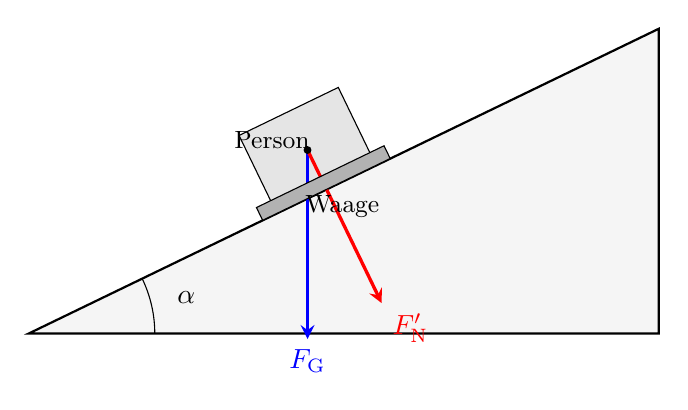
\begin{tikzpicture}[>=stealth]
 \draw[thick, fill=gray!8] (0,0) -- (8.00,0) -- (8.00,3.87) -- cycle;
 \draw (1.6,0) arc (0:25.84:1.6);
 \node at (2.00,0.46) {$\alpha$};
 \begin{scope}[shift={(3.78,1.83)}, rotate=25.84]
  \draw[fill=gray!20] (-0.7,0) rectangle (0.7,1.1);
  \node[font=\small] at (-0.35,0.86) {Person};
 \end{scope}
 \draw[->, very thick, blue] (3.54,2.33) -- ++(-90.00:2.40) node[anchor=north] {$F_\mathrm{G}$};
 \draw[->, very thick, red] (3.54,2.33) -- ++(-64.16:2.16) node[anchor=north west] {$F_\mathrm{N}^\prime$};
 \fill (3.54,2.33) circle (0.05);
 \begin{scope}[shift={(3.78,1.83)}, rotate=25.84] \draw[fill=gray!60] (-0.9,0) rectangle (0.9,0.18); \node[font=\small, anchor=north] at (0.2,-0.05) {Waage}; \end{scope}
\end{tikzpicture}
\end{center}

Eine Personenwaage misst die Kraft, mit der die Person senkrecht auf die Waagplatte drückt (die Gegenkraft $F_\mathrm{N}^\prime$ der Normalkraft). Diese Kraft rechnet sie mit dem Ortsfaktor $g$ in eine Masse um. Auf der geneigten Waage drückt die Person nur mit der Komponente der Gewichtskraft senkrecht zur Platte:
\begin{align}
 F_\mathrm{N}^\prime &= m\,g\cos\alpha
\end{align}
Die angezeigte Masse ist also um den Faktor $\cos\alpha$ zu klein. Für eine um $p = \pReO$ zu kleine Anzeige gilt
\begin{align}
 \cos\alpha &= 1-p \\
 \alpha &= \wiF = \wi \approx \result{\wiP{0}{2}}
\end{align}

Die Waage misst also eigentlich eine Kraft, nämlich die Normalkraft, und nicht die Masse. Auf dem Mond würde sie deshalb ebenfalls zu wenig anzeigen. Eine Balkenwaage (Hebelwaage) vergleicht dagegen die Gewichtskräfte der zu wägenden Masse und von Wägestücken bekannter Masse; da beide gleich stark von $g$ abhängen, misst sie tatsächlich die Masse.
